% \chapter{Datový model}
% Chceme-li dle kompetencí vyhledávat je třeba definovat, jaká data potřebujeme. Druhá neméně důležitá otázka je, jak nejlépe tyto data reprezentovat v strojově čitelné podobě. Na obě tyto otázky se pokusíme odpovědět v této kapitole.
\chapter{Konceptuální datový model} \label{chap:data_model} 
V následující kapitole rozebereme zkoumanou doménu. Tím mimo jiného odpovíme i na otázku \textit{Která data potřebujeme?} (definovanou v kapitole č. \ref{chap:decompisition}).
Ujasníme si, které entity se v naší doméně vyskytují, jaké mají vlastnosti a jaké jsou mezi nimi vztahy.\par 
\noindent Ze zadání vyplývají základní řešené entity – osoby, pracoviště, kompetence. 
% Všechny tyto se vždy vztahují k dané organizaci, ve které vytváříme databázi kompetencí.
\section{Osoby}
% Osoby .
% Uvádíme i atributy, které se obecně považují za osobní údaje. Tyto údaje jsou typicky uchovány v interní databázi organizace a není třeba s nimi manipulovat. Pro naše účely poslouží jen obecný identifikátor v rámci organizace.
% \par
\paragraph{Vlastnosti:}
\begin{itemize}
\item Identifikátor v rámci organizace
\item Jméno
\item Příjmení
\item Pracoviště
\item \textit{Abstraktní hodnocení} - vědecké (např. h-index), pracovní (roky zkušeností) a jiné
\item Znalosti a dovednosti
\item Osobnost - společenské vnímáni, vnímání sebe sama (viz obr. č. \ref{fig:competence_structure} pod hladinou)
\end{itemize}
\section{Pracoviště}
% Jedná se o množinu osob s definovaným vedoucím.\par
\paragraph{Vlastnosti:}
\begin{itemize}
\item Identifikátor v rámci organizace
\item Název
\item Skupina osob
\item Vedoucí
\end{itemize}
\section{Kompetence}
Kompetence je klíčovým prvkem naší domény, její popis je úzce provázán s její reprezentací. To je důvod, proč nemusí být na první pohled zjevné, jak budou její atributy vypadat. Jedná se však jen o konceptuální model, podrobnosti týkající se reprezentace těchto dat připojíme v pozdějších kapitolách. \par
\paragraph{Vlastnosti:}
\begin{itemize}
\item Formální název popř. popis
\item Zdroje - znalosti/dovednosti, povahové rysy (viz obr. č. \ref{fig:competence_structure})
\end{itemize}
\section{Diagram konceptuálního modelu}
Diagram (příloha č. \ref{fig:conceptual_appendix}) zobrazuje vztahy entit mezi sebou a násobnosti těchto vztahů. \par
\noindent Levá část diagramu týkající se osobnosti je pouze schematicky naznačena bez hlubšího rozebrání její vnitřní struktury. Tuto část bereme spíše jako tzv.~\textit{černou skřínku}, neuváděli jsme ani násobnosti vazeb.\par
Cílem konceptuálního modelu je co nejlépe zachytit naší interpretaci skutečnosti. Interpretací může existovat nespočet, tento náš model je výsledkem několika iterací.\par
% Jedná se pouze o konceptuální model, jde tedy výhradně o model interpretace reálného světa, ne o technickou reprezentaci.
% \begin{figure}[htbp!]
% 	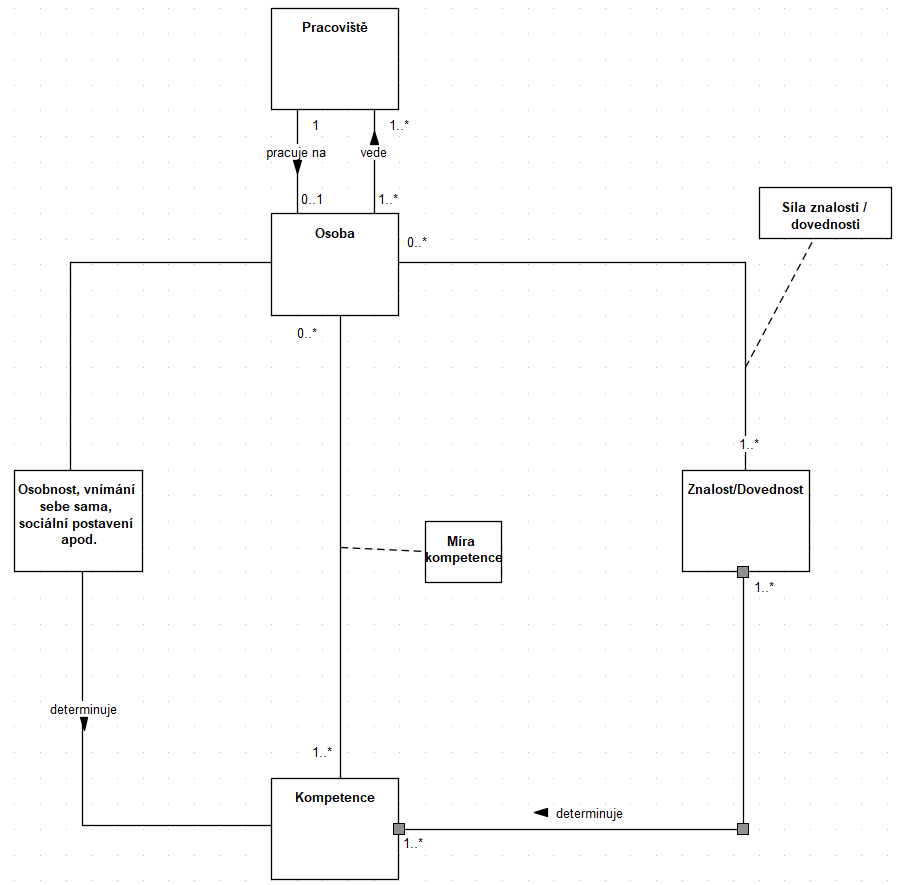
\includegraphics[width=\linewidth]{img/data_diagram.png}
% 	\caption{Diagram konceptuálního modelu}
% 	\label{fig:conceptual_inline}
% \end{figure}
\section{Shrnutí}
Účelem této sekce bylo odpovědět na otázku \textit{Která data potřebujeme?}. Víme, že budeme muset získávat data o osobách, pracovištích a kompetencích. Přibližně víme i jaké atributy můžeme u těchto entit očekávat, z čeho se dále skládají a jaké jsou mezi nimi vazby. Nedozvěděli jsme se přesnou povahu dat, například jejich formu, to rozebereme až v následujících kapitolách.

